% boosting.tex
% Jeremy Barnes, 29/8/1999
% $Id$

% The chapter of my thesis on Boosting
% Still theory

\chapter{AdaBoost and boosting algorithms}
\label{chapter:boosting}

Boosting algorithms are a very important recent development in machine
learning that has significantly altered the field.  The name
``Boosting'' is applied to a range of  machine learning algorithms,
all of which combine many weak hypotheses to form a ``strong''
hypothesis that significantly outperforms them. 

In this chapter we describe the classic algorithm \emph{AdaBoost}
developed by Freund and Schapire \cite{Freund96}.  Results on its
properties and generalisation performance are also presented.  We then
look at AdaBoost as optimisation via gradient descent of a cost
function, and derive a result which shows this to be the case.  We
digress slightly to look at \emph{normed} boosting algorithms, a minor
modification, and conclude by considering the problem of overfitting
as applied to boosting algorithms.

\section{The AdaBoost algorithm}

We first describe the AdaBoost algorithm, first published by Freund
and Schapire \cite{Freund96}.  In essence, this algorithm
``bootstraps'' itself onto another learning algorithm (the \emph{weak
learning algorithm}) and improves performance by using a ``voting
committee'' (linear combination) of weak learning hypotheses.

AdaBoost performs \emph{very} well; its combined hypotheses generally
perform significantly better than \emph{any} non-boosted algorithm.
This is particularly true for reliable (low-noise) data.  Even
the simplest of weak algorithms, when ``boosted'', will usually
outperform the best unboosted algorithms.
\footnote{As a result, the focus of recent research effort has shifted
from the development of \emph{learning} algorithms (which are all more 
or less equivalent when boosted) to the development of better
\emph{boosting} algorithms.}

We consider questions of how and why AdaBoost works; in
particular how it chooses the optimal linear combination of
classifiers from the very large set of possible linear combinations.

Figure \ref{fig:boosting algorithm} gives an explicit description of
AdaBoost.  The key features are:
%
\begin{enumerate}
\item	The AdaBoost algorithm operates in iterations.  During
	iteration $t+1$, one classifier $h_{t+1}$ is added to the combined
	hypothesis $F_{t}$, to give $F_{t+1} = F_t + b_t h_{t+1}.$
\item	The weight $b_t$ of each weak hypothesis (the \emph{classifier
	weight}) depends upon the weighted empirirical risk
	(definition \ref{def:weighted empirical risk}) of that
	classifier over the training dataset.  Section
	\ref{sec:classifier weights} describes these classifier
	weights in more detail.
\item	Each sample in the training dataset is given a weight
	(\emph{sample weight}) which is modified depending upon how
	``hard'' that sample is to classify.  Section \ref{sec:sample
	weights} describes these sample weights in more detail.
\end{enumerate}

The notation $w_{t,i}$ denotes the weight of sample $i$ at iteration
$t$.  The process of training AdaBoost for one iteration is denoted $F_t
\trainboost F_{t+1}$.   Two AdaBoost hypotheses are said to be
\emph{equivalent} ($\equiv$) if they produce the same output for all
input, even if their internal state ($b$ and $w$ values) are not
identical.

\begin{linefigure}
\label{fig:boosting algorithm}
\noindent{\bf Input:} $m$ examples $X = ((\bfx_1, y_1), \ldots, (\bfx_l,
y_m))$ and a weak learning algorithm $\bbW$
\par
\noindent{\bf Initialisation:} $F_0(\bfx) = 0$; $\bfw_0 : w_{0,i} = 1/m$ for
$i=1 \ldots m$ 
\par
\noindent {\bf Do for} $t=1 \ldots T$:
\par
\noindent Update $F_t \trainboost F_{t+1}$: 
\par
\begin{enumerate}

\item	Train weak learner $\bbW$ on the weighted sample set 
	$(\bfx_1, y_1, w_{t,1} \ldots (\bfx_m, y_m, w_{t,m})$
	and obtain weak learner $h_t : \calI \rightarrow \{\pm 1\}$

\item	Calculate the weighted empirical risk (training error
	$\epsilon_t$) of $h_t$: 
	%
	\begin{equation}
	\epsilon_t = R_{\emp}^{\bfw_t}(h) = \sum_{j : h(\bfx_j) \neq
	y_j} w_{t,j}
	\end{equation}

	If $\epsilon_t = 0$ (a single weak learner can correctly learn
	the relationship) or $\epsilon_t \geq 1/2$ (the weak
	learner is performing as badly as random guessing) then abort
	the training process, with $F_{t+1} = F_{t}$.

\item	Calculate the classifier weight $b_t$:
	\begin{equation}
	b_t = - \frac{1}{2} \log \frac{\epsilon_t}{1 - \epsilon_t}
	\end{equation}

\item	Update the sample weights $\bfw_t \Rightarrow \bfw_{t+1}$:
	%
	\begin{equation}
	w_{t+1, i} = \left\{
	\begin{array}{ll}
		\frac{w_{t, i}}{Z_t} \exp \left\{ b_t \right\}&	\qquad
		\qquad \mbox{if  $f_t(\bfx_i) = y_i$} \\
		\frac{w_{t, i}}{Z_t} \exp \left\{ -b_t \right\} & \qquad \qquad
		\mbox{otherwise} \\
	\end{array} \right.
	\label{eqn:sample weight update}
	\end{equation}

	where $Z_t$ is a normalisation constant, such that
	$\sum_{i=1}^{m} w_{t, i} = 1$
\end{enumerate}

\par
\noindent {\bf Output:} 
\begin{equation}
H_T(\bfx) = \sign (F_T(\bfx)) = \sign \left\{ \sum_{i=1}^T b_i
h_i(\bfx) \right\} 
\end{equation}
\caption{The AdaBoost algorithm $\bbB$}
\end{linefigure}


\subsection{Classifier weights}
\label{sec:classifier weights}

AdaBoost's training process is divided into iterations.  On iteration
$t$, one weak learner $h_t(\cdot)$ is added to the linear
combination ($h_t$ is chosen by the weak learning algorithm).  The
coefficient $b_t$ of $h_t$ is calculated from the 
training error $\epsilon_t$ of $h_t$ as 
%
\begin{equation}
b_t = - \log \frac{\epsilon_t}{1 - \epsilon_t}
\label{eqn:theory:bt}
\end{equation}
%
which is plotted in figure \ref{fig:b function}.

\begin{linefigure}
\begin{center}
\includegraphics{figures/classifier_weights.epsg}
\end{center}
\begin{capt}{Classifier weights against weighted training error}{fig:b
function}
When $\epsilon_t = 1/2$, the classifier only does as well as random
guessing, and $b_t = 0$.  As $\epsilon_t$ approaches zero, $b_t$
increases without bound.  The effect is that $F$ becomes dominated by
those weak hypotheses that performed well on the training samples
(training is halted if $\epsilon_t = 0$ or $\epsilon_t \geq
1/2$).
\end{capt}
\end{linefigure}


\subsection{Sample weights}
\label{sec:sample weights}

Each sample in the training set has a corresponding weight $w_j$ which
is updated to reflect the difficulty of that sample.  On each iteration the
weights of samples which $h_t$ classified incorrectly are increased
(scaled by $\exp \{ -b_t \}$); the whole lot are then normalised.
This function has the following effect on the distribution of weights
(illustrated in figure \ref{fig:sample weights}):

\begin{itemize}
\item	Training samples which are misclassified often, or are one of 
	few points to get misclassified, increase their proportion of
	the weight (they are identified as ``hard samples'');
\item	Other samples decrease their proportion of the weight, and are
	effectively identified as ``easy'' samples.
\end{itemize}

\begin{linefigure}
\begin{center}
\includegraphics{figures/sample_weights.epsg}
\end{center}
\begin{capt}{Evolution of sample weights}{fig:sample weights}
The figure shows the evolution of the sample weights from (a) 10
iterations to (b) 100 iterations of boosting over a set of training
data in $\bbR^2$.  The sample weight at a point is proportional to the
intensity of the dot.  It can be seen that as $t \rightarrow \infty$,
the ``easy'' samples (far from the decision boundary) lose weight
relative to the ``hard'' samples.
\end{capt}
\end{linefigure}

The overall effect is for those samples near the decision boundary to
increase in weight, and those far from it to decrease.  This forces
the algorithm to concentrate on the hard samples, and is one reason
why it works well on low-noise datasets.  Unfortunately, those samples
corrupted by noise are usually hard also, and concentrating on those
is not desirable.


\section{Boosting as gradient descent}
\label{sec:theory:gradient descent}

Recent work has shown boosting to be an implementation of a gradient
descent algorithm in an inner product space
\cite{Mason99}.%
\footnote{This discussion follows \cite{Mason99} rather closely with
some changes in notation and omission of details such as stopping
criteria.}
An inner product space requires both a universal set $\mathcal{X}$ and
an inner product operator \ip{\cdot}{\cdot}.  We define
%
\begin{equation}
\calX = 
\mathrm{co} (\calH) \doteq
 \bigcup _{n \in \mathbb{N}}
\left\{
 \sum_{i=1}^{n}
  b_i
f_i : f_1, \ldots, f_n \in \calH, \quad
 b_1, \ldots, b_n > 0, \quad
 \sum_{i=1}^{n} b_i = 1
\right\} \cup \emptyset
\end{equation}
%
(which is the convex hull of \calH), and
%
\begin{equation}
\ip{F}{G} = \frac{1}{m} \sum_{i=1}^{m} F(\bfx_i)G(\bfx_i) \qquad
F, G \in \calX
\label{eqn:inner product definition}
\end{equation}
%
where it should be noted that $\ip{\cdot}{\cdot}$ implicitly depends
upon a series of training samples $X = ((\bfx_1, y_1), \ldots,
(\bfx_m, y_m))$.

We furthermore define the \emph{cost functional}
%
\begin{equation}
\label{eqn:gradient descent cost functional}
C(F) = \frac{1}{m} \sum_{i=1}^{m} c(y_i F(\bfx_i))
\end{equation}
%
which sums another function $c$ over the \emph{margin} of all training
samples.

At iteration $t$ of gradient descent, we wish to choose a hypothesis $h_t$ and
a weight $b_t$ such that $C(F + b_t h_t) < C(F)$.  We do not choose
$h_t$ directly, however--that is done by the weaklearner--instead, we
manipulate the sample weights $\bfw_t$ in such a manner that (as we
will see) the weaklearner chooses the ``right'' $h_t$ for us.  The
right $h_t$ is the one that leads to the steepest reduction in the cost
function:
%
\begin{equation}
h_t^{\ast} = -\nabla C(F)(\bfx) = \left. \frac{\partial C(F + \alpha
1_{\bfx})}{\partial \alpha} \right|_{\alpha = 0}
\label{eqn:functional derivative}
\end{equation}
%
where $1_{\bfx}$ is the indicator function of $\bfx$; this is
necessary as we can only evaluate (\ref{eqn:functional derivative})
where we have a sample.  Since the optimal $h_t^{\ast}$ will not
necessarily be in $\calH$, we choose the $h_t \in \calH$ with the
greatest inner product $\ip{-\nabla C(F)}{h_t^{\ast}}$.  More
specifically, using the inner product space and cost functions we have
chosen we are maximising 
%
\begin{equation}
- \ip{\nabla C(F)}{f} = - \frac{1}{m^2} \sum_{i=1}^{m} y_i f(\bfx_i)
  C'(y_i F(\bfx_i))
\label{eqn:function to maximise}
\end{equation}
%
The following theorem states that the \emph{weighted empirical risk}
$R_{\emp}^{w}$ (section \ref{sec:weighted empirical risk}) is the
``right'' form of risk to minimise, and gives the weights $\bfw_t$.

\begin{theorem}[Weighted empirical risk minimisation]
Maximising (\ref{eqn:function to maximise}) is equivalent to
minimising the weighted empirical risk
%
\begin{equation}
R_{\emp}^{w_{|t}} = \sum_{i:y_i \neq h(\bfx_i)}^{m} w_{i|t}
\end{equation}
%
where $\bfw_{t}$ is given by
%
\begin{equation}
w_{t,i} = \frac{C'(y_i \: F_t (\bfx_i))}{\sum_{j=1}^{m} C'(y_j \:
F(\bfx_j))}
\label{eqn:gradient sample weights}
\end{equation}
\end{theorem}
\proof See \cite{Mason99}.  We assume that $C(\alpha)$ is
monotonically decreasing with respect to an increasing $\alpha$; the
result follows easily from this assumption.

Having chosen our direction $h_t$, we now choose a step size $b_t$.
AdaBoost uses a line search for the minimum of the cost functional
along the line
%
\begin{equation}
b_t = \arg \min_{b_t} \sum_{i=1}^{m} C(y_i F(\bfx_i) + y_i b_t h_t(\bfx_i))
\end{equation}
%
The line search is illustrated in figure \ref{fig:gradient descent}.

\begin{linefigure}
\begin{center}
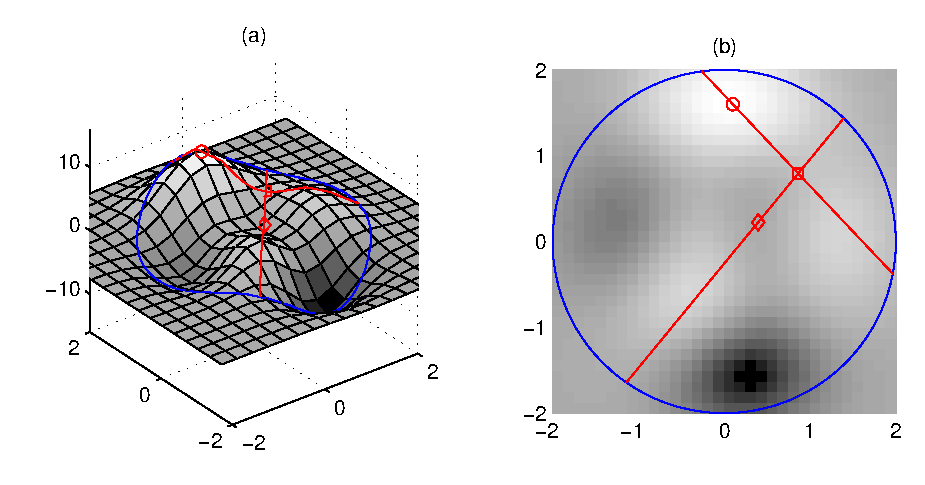
\includegraphics{figures/descent.epsg}
\end{center}
\begin{capt}{Schematic representation of gradient
descent.}{fig:gradient descent}
Points within the circle are in \calH, the height of the surface
the value of (\ref{eqn:theory:cost function}) at that point.  (a) is a
3D view, (b) is top view. Lines show line searches; markers
minimums.  We descend from $\circ$ through $\Box$ to $\Diamond$, where
the algorithm terminates due to a local minima.
\end{capt}
\end{linefigure}

We will now show that AdaBoost implements gradient descent using the
cost function $c(\alpha) = e^{-\alpha}$.  We do this by showing that
gradient descent produces the same $b_t$ and $\bfw_t$ values as AdaBoost.

\begin{theorem}[AdaBoost implements gradient descent]
The AdaBoost algorithm implements gradient descent over a margin cost
function
%
\begin{equation}
c(\alpha) = e^{-\alpha}
\end{equation}
\end{theorem}

\proof We outline a skeleton, ignoring initial conditions and the
stopping conditions.  We will show that, given a state at iteration
$t$, then boosting and gradient descent produce identical states at
iteration $t+1$.

Once the weaklearner has chosen $h_{t+1}$ using weighted empirical risk
minimisation, we choose $w_{t+1}$ to minimise the cost functional
along the line $F_t + b_{t+1} h_{t+1}$.  The value of the cost
functional along this line is
%
\begin{equation}
C = \sum_{i=1}^{m} c \left( y_i F_t(\bfx_i) + y_i b_{t+1}
h_{t+1}(\bfx_i) \right)
\end{equation}
%
Substituting in $c(F(\bfx_i)) = e^{-yF(\bfx_i)}$, we obtain
%
\begin{equation}
C = \sum_{i=1}^{m} \exp \left\{ y_i F_t(\bfx_i) + y_i b_{t+1}
h_{t+1}(\bfx_i) \right\}
\label{eqn:cost functional along line}
\end{equation}
%
We minimise (\ref{eqn:cost functional along line}) by
differentiating and setting the derivative to zero.  The task is
simplified considerably by noting that only the second half of the
exponential term is variable with $b_{t+1}$.  The result is that
%
\begin{eqnarray}
\label{eqn:differentiate}
\frac{\partial C}{\partial b_{t+1}} &
= & \sum_{i=1}^{m} \frac{\partial}{\partial b_{t+1}}
\exp \left\{ y_i F_t(\bfx_i) + y_i b_{t+1}
h_{t+1}(\bfx_i) \right\} \nonumber \\
& = & \sum_{i=1}^{m} y_i \exp \left\{ y_i F_t(\bfx_i) + y_i b_{t+1}
h_{t+1}(\bfx_i) \right\} 
\end{eqnarray}
%
We make several simplifications.  Noting that
%
\begin{equation}
y_i h_{t+1}(\bfx_i) = \left\{ 
	\begin{array}{ll}
	1 &	\qquad \mbox{if $y_i = h_{t+1}(\bfx_i)$} \\
	-1 &	\qquad \mbox{if $y_i \neq h_{t+1}(\bfx_i)$}
	\end{array}
\right.
\end{equation}
%
and that $w_{t,i} = k \exp \{ -y_i F_t(x_i) \}$ where $k$ is some
(normalising) constant, we recast (\ref{eqn:differentiate}) into
the form 
%
\begin{equation}
\underbrace{
	\frac{\sum_{i : y_i = f_{t+1}(\bfx_i)} w_{i|t}}
	     {\sum_{i : y_i \neq f_{t+1}(\bfx_i)} w_{i|t}}
}_{\epsilon_t}
= \exp \left\{ 2 b_{t+1} \right\} 
\end{equation}
%
from which it is a simple transformation to obtain
(\ref{eqn:theory:bt}).  Thus, we update our state in the same manner
as AdaBoost; therefore AdaBoost implements gradient descent.

The cost functional $c(\alpha) = e^{-\alpha}$ is an approximation to
the misclassification risk (\ref{eqn:misclassification risk}) that is
differentiable at all points and leads to a closed-form solution for
the step size.  It is plotted in figure \ref{fig:cost functional
approximation}.  Other approximations have been used; see Mason
et. al. \cite{Mason99} for details.

\begin{linefigure}
\begin{center}
\includegraphics{figures/cost_approx.epsg}
\end{center}
\begin{capt}{Approximation to the misclassification risk
function}{fig:cost functional}
The misclassification risk is plotted in the dotted line, with the
AdaBoost approximation plotted in the solid line.  It is clear that
the effect of this cost function will be to maximise the margins of
the samples.
\end{capt}
\end{linefigure}

\subsection{Modifying gradient descent}

In this section, we have shown that the AdaBoost algorithm implements
gradient descent.  There are four degrees of freedom which can be
exploited to produce modified versions of gradient descent:
%
\begin{enumerate}
\item	What is our universal set? (AdaBoost: $\co(\calH)$)
\item	What is our inner product? (AdaBoost: equation (\ref{eqn:inner
	product definition}))
\item	What is our cost function? (AdaBoost: $c(\alpha) =
	e^{-\alpha}$)
\item	How do we choose a step size? (AdaBoost: line search).
\end{enumerate}
%
In chapter \ref{chapter:development} we will consider changing some of
these to implement algorithms with desirable properties.


\section{AdaBoost and Boosting algorithms}

Until this point we have only considered the AdaBoost algorithm.  We
now extend our scope to other AdaBoost-like algorithms.  These
algorithms are termed ``boosting algorithms''.

There has recently been some debate over what constitutes a ``boosting
algorithm''; see for example Duffy and Helmbold \cite{Duffy99} who
adopt quite a restrictive definition.  In this thesis, we take a very
broad definition:

\begin{definition}[A boosting algorithm]
Any learning machine that constructs a hypothesis that is a linear
combination of base hypotheses by leveraging another learning machine
in an interative manner is a boosting algorithm.
\end{definition}

In particular, we don't require that the training error be guaranteed
to reach zero.  All algorithms considered in this thesis are,
according to definition \ref{def:boosting}, boosting algorithms.


\section{Properties of the AdaBoost and boosting algorithms}

We have covered the \emph{form} of the AdaBoost algorithm quite
extensively.  We now cover the \emph{function} of the algorithm, so
that we have a basis for comparison.

\subsection{Convergence properties}

This theorem provides two results.  The first, applicable to any
algorithm that implements gradient descent, shows that under certain
conditions on the cost function and step sizes the 
e main result of this section is a theorem that the empirical risk
(training error) of boosting will converge to zero if the algorithm is
trained for long enough.

\begin{theorem}[AdaBoost converges to zero training error in finite
time \cite{Freund97}]
\label{thm:AdaBoost training error convergence}
Suppose that the AdaBoost algorithm $\bbB$ operating on weaklearning
algorithm $\bbW$ generates hypotheses $h_t$ with training errors
$\epsilon_1 \ldots \epsilon_T$ over a training set $X$.  Furthermore,
assume that each $\epsilon_t < 1/2$, and let $\beta_t = 1/2 -
\epsilon_t$.  Then the empirical risk of the \emph{combined}
hypothesis $H_t = \sign(F_t)$ is bounded by
%
\begin{equation}
R_{\emp}(H_t) \leq \prod_{t=1}^{T} \sqrt{1 - 4 \beta_t^2} \leq \exp
\left\{ - 2 \sum_{t=1}^T \beta_T^2 \right\}
\end{equation}
\end{theorem}

\proof The straightforward proof of this theorem is contained in
\cite{Freund97}.

\begin{theorem}[Sum of AdaBoost classifier weights is unbounded]
\label{thm:increasing classifier weights}
\todo{Finish this theorem.  It must be published somewhere...}
\end{theorem}

\proof It suffices to show that, for a constant $\epsilon > 0$ that
there is always an iteration $t + \delta t$ such that the weight...


The following theorem shows that the total weight of the boosting
algorithm is unbounded as the number of iterations increases.  It is
used to prove results on the minimum margin and final training error
of boosting.

\begin{theorem}
The size of the $b$ weight vector, $\|b\| \rightarrow \infty$
as $t \rightarrow \infty$ (assuming the boosting algorithm doesn't
terminate).

\proof ?
\end{theorem}



\subsection{AdaBoost maximises the minimum margin}

This section introduces several theorems which together show that
AdaBoost chooses the linear combination that maximises the minimum
margin over its training samples.

\begin{theorem}[AdaBoost maximises the minimum margin]
\todo{Rework this theorem!}
Given a particular learning algorithm $F$ and a training
set $S$, define the minimum margin as
\[
m_{\min} = min_{\{x,y\} \in S} y_i F(x_i)
\]
Then the boosting algorithm will converge as $t \rightarrow \infty$ to
the solution which maximised the minimum margin.

\proof For boosting we can write $F_t = b_1 f_1 + \cdots + b_t f_t$.
Then defining our \emph{normalised hypotheses} $\bar{f}_i$ as
\[
\bar{f} = \frac{b_i f_i}{\|b\|}
\]
such that $\hat{F}_t = \bar{f}_1 + \cdots + \bar{f}_t$, we can write
our cost function (reference?) as 
\[
C(b, S) = \sum_{i=1}^{m} \exp\{-y_i \bar{F}_t(x_i)\}^{\|b\|}
\]
We already know from the gradient descent theory (reference?) that we
are trying to minimise the cost function.  Now as $\|b\| \rightarrow
\infty$ (from the previous theorem) the largest value of $\exp\{-y_i
\bar{F}_t(x_i)\}$ will dominate, and so $C(b, S) \rightarrow exp\{\max
-y_i \bar{F}_t(x_i)\}$.  Thus, by minimising $C(b, S)$, we are making
$\min y_i \bar{F}_t(x_i)$ as large as possible; that is we are
maximising the minimum margin.
\end{theorem}


\subsection{Invariance of AdaBoost to uniform scaling of classifer
weights}

We present here an obvious theorem about the invariance of hypothesis
weights.  It will be used in chapter \ref{chapter:results}.

\begin{theorem}
The hypothesis returned by the AdaBoost is independent of a 
scaling of the $b$ values.  Given an unthresholded hypothesis $F$ and
a constant $\alpha > 0$,
%
\begin{equation}
H = \sign(F) \equiv H' = \sign(\alpha F) 
\end{equation}
\end{theorem}

\proof This follows easily from the fact that the sign function is
independent of a scaling of the $b$ values.



\section{Performance bounds for Boosting}

The following theorem appears in Schapire et. al \cite{Schapire97}.

\begin{theorem}[Performance bound for boosting ($p$=1)]

There is a constant $c$ such that a combined hypothesis $H = \sign(F)$
generated by the AdaBoost algorithm $\bbB$ from a base class $\calH$
with VC dimension $d$, with probability at least $1 - \delta$ over $m$
independent training samples has true risk bounded by 
\begin{equation}
R(F) \leq R_{\emp}^{\gamma}(F) + \sqrt{\frac{c}{m} \left[ \frac{d
\ln^2 (m/d)}{\gamma^2} + \ln(1/\delta) \right] }
\end{equation}
\end{theorem}


\section{Overfitting}
\label{sec:boost overfitting}

Initial experiments with AdaBoost indicated that the algorithm was
remarkably resistant to overfitting, despite the unlimited complexity
of the hypothesis space \cite{Freund96}.
However, further experiments \cite{Grove98, Bauer99} revealed that
training to $10^4$ to $10^6$ iterations, or adding label noise, would
often induce overfitting.  Figure \ref{fig:overfitting graphs} shows some
examples of the effect.  There have been several studies into the
characteristics of AdaBoost that lead to overfitting \cite{Schapire97,
Grove98, Ratsch98}.  A largely intuitive survey of the characteristics
of AdaBoost that lead to overiftting is presented here. 

\begin{linefigure}
\begin{center}
\includegraphics{figures/boost_overfitting.epsg}
\end{center}
\begin{capt}{Experimental results for Boosting showing overfitting}
Three plots of test/training error vs iteration number for Boosting.
The dataset used was the ``ring'' distribution (see chapter
\ref{chapter:method}) with 50 samples.  Mild overfitting is visible on
the 20\% noise plot and becomes more pronounced as the level of noise
increases.
\end{capt}
\end{linefigure}

That overfitting occurs in AdaBoost follows from the property that
AdaBoost maximises the minimum margin (theorem
\ref{thm:max-min-margin}).  Intuitively, this property causes the
AdaBoost algorithm to concentrate on a few hard samples.
Unfortunately, in a noisy dataset, these samples are usually all
noisy.  Some algorithms are described in the next section that 

\section{Previous work on regularising AdaBoost}

Following the discovery that AdaBoost operated by maximising the
minimum margin, several efforts were made to regularise AdaBoost to
avoid overfitting.  Algorithms such as \emph{soft margins}
\cite{Ratsch98} explicitly allow a certain number of training samples
to have a small or negative margin; while algorithms such as DOOM and
DOOM II \cite{Mason99a, Mason99b} do this implicitly by flattening out
the cost function (figure \ref{fig:cost functional}) for low and
negative margins.  These approaches have been quite successful, both
outperforming AdaBoost under certain conditions (in particular on
noisy data).


\section{Normed boosting algorithms}

Mason et al. \cite{Mason99a} have studied another modification to
AdaBoost, where theclassifier weights are \emph{normalised at each
iteration}.  After $b_t$ is calculated for iteration $t$, the entire
set of classifier weights $b$ are normalised:
%
\begin{equation}
b_{i} \Leftarrow \frac{b_i}{\| \mathbf{b} \|_p} \qquad \mbox{for} i=1
\ldots t
\end{equation}
%
where the norm is chosen via the $p$ parameter.%
\footnote{Mason et. al. considered mainly $p \in \{ 1,2 \}$ in
\cite{Mason99a}.}

While it can be shown that these algorithms converge to the global
minimum of the gradient descent cost functional (\ref{eqn:gradient
descent cost functional}), they do \emph{not} have the property of
guaranteed convergence to zero training error (theorem
\ref{thm:AdaBoost training error convergence}); the reason being that 
$\sum_{i=1}^t b'_{t,i}$ is bounded above (theorem \ref{thm:increasing
classifier weights} does not hold).  As results in chapter
\ref{chapter:results} and the discussion in section \ref{sec:boost
overfitting} indicate, an algorithm does not have to converge to zero
training error to generalise well.

One of the algorithms developed in chapter \ref{chapter:pboosting} is
a generalisation of the normed boosting algorithm described in this
section, where the value of $p$ is unrestricted.





